\chapter{Военные корабли и их операторы}
\label{ch:ships-chapter}

Глава посвящена отечественным и зарубежным кораблям. Они могут иметь как военное, так и гражданское назначение. Гражданские суда используются в грузоперевозках, рыболовстве, туризме, разведке полезных ископаемых, спасательных работах, а также в спортивных, культурных и других целях. Для хранения информации о судах и других объектах ведутся базы знаний. Одной из таких баз знаний являются Викиданные. В этой главе изучены хранимык в Викиданных объекты кораблей и проведена оценке качества и полноты их описания.


\begin{marginfigure}[0.0cm]
  {
    \setlength{\fboxsep}{0pt}%
    \setlength{\fboxrule}{1pt}%
    \fcolorbox{gray}{gray}{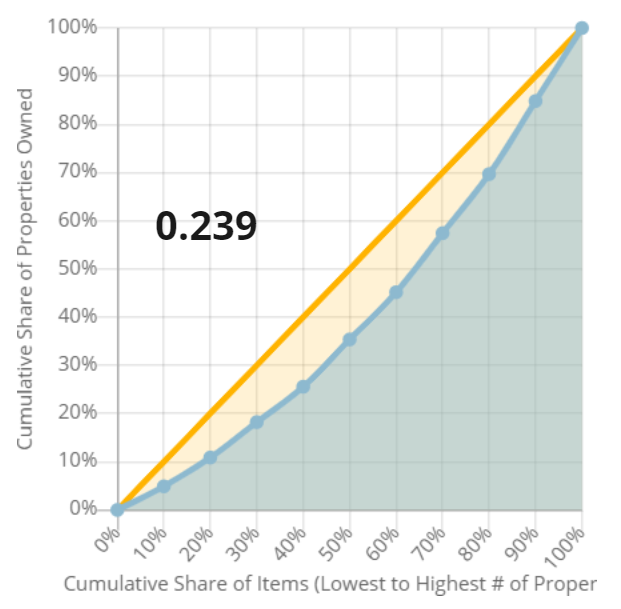
\includegraphics{chapter/ship/Russian_ships_topic_imbalance.png}}
  }
  \caption{
    График равномерности заполнения по числу свойств объекта Викиданных \href{https://www.wikidata.org/wiki/Q11446}{корабль (Q11446)}, коэффициент Джини равен 0.239. Данные получены с помощью сервиса ProWD.id, 2020 год. График и коэффициент Джини показывают низкую равномерность заполнения свойств.
    }%
    \label{fig:prowd_ships-unbalanced}%
  \end{marginfigure}

\section{Список кораблей}

\marginnote{
\href{https://www.wikidata.org/wiki/Q11446}{Корабль (Q11446)} -- это крупное морское судно.

Исследуемые свойства:
\begin{itemize}
  \item\href{https://www.wikidata.org/wiki/Property:P31}{Экземпляр (P31)}.
  \item\href{https://www.wikidata.org/wiki/Property:P137}{Оператор (P137)}.
  \item\href{https://www.wikidata.org/wiki/Property:P17}{Государство (P17)}.
  \item\href{https://www.wikidata.org/wiki/Property:P607}{Конфликт (P607)}
\end{itemize}
}

Построим список всех кораблей (см. листинг \ref{lst:ships_ru}).

\begin{lstlisting}[ language=SPARQL, caption={{\href{https://w.wiki/koL}{Список кораблей}}\protect\footnotemark}, label=lst:ships_ru, ]
#List of ship
SELECT ?ship ?shipLabel
WHERE
{
  ?ship wdt:P31 wd:Q11446. # instance of ship
  SERVICE wikibase:label { bd:serviceParam wikibase:language "ru". }
}
\end{lstlisting}
\footnotetext{Найдено \num{19820} кораблей в 2017 и \num{50681} в 2020. Ссылка на SPARQL-запрос: \href{https://w.wiki/koL}{https://w.wiki/koL}. }

По данным ProWD больше всего свойств (34) имеет \href{https://www.wikidata.org/wiki/Q281147}{ледокол Красин}\cite{ProWD_ru_ships}.

Составим список кораблей, операторы которых находятся или находились в России, СССР или Российской империи (см. листинг \ref{lst:ships_with_ru_op}).

\begin{lstlisting}[ language=SPARQL, caption={\href{https://w.wiki/koN}{Cписок кораблей, операторы которых находятся или находились в России, СССР или Российской Империи}}, label=lst:ships_with_ru_op ]
#List of ship from Russia, Soviet Union and Russian Empire
SELECT ?ship ?shipLabel
WHERE
{
  ?ship wdt:P31 wd:Q11446. # instance of ship
                                    # ships belongs to:
  { ?ship wdt:P137/wdt:P17 wd:Q34266 } UNION  # Russian Empire
  { ?ship wdt:P137/wdt:P17 wd:Q15180 } UNION  # Soviet Union
  { ?ship wdt:P137/wdt:P17 wd:Q159 }.         # Russia
  SERVICE wikibase:label { bd:serviceParam wikibase:language "ru". }
}
\end{lstlisting}
\footnotetext{Найдено 579 кораблей в 2020 г. Ссылка на SPARQL-запрос: \href{https://w.wiki/koN}{https://w.wiki/koN}.}

% \section{Плохие и хорошие примеры}

% Хорошие примеры объектов кораблей на сайте Викиданных: \href{https://www.wikidata.org/wiki/Q613128}{SMS Moltke}, \href{https://www.wikidata.org/wiki/Q596282}{HMS Hermes}, \href{https://www.wikidata.org/wiki/Q596282}{HMS Barham}.

% Плохими примерами объектов кораблей на сайте Викиданных были: \href{https://www.wikidata.org/wiki/Q4264229}{Лихой}, \href{https://www.wikidata.org/wiki/Q18816894}{Николай Вилков}, \href{https://www.wikidata.org/wiki/Q4528362}{Щ-310}.

\section{Полнота Викиданных}

Поиск точного количества кораблей в мире — трудная задача. Ведь данные о некоторых из них являются совершенно секретными, какие-то же — это частные судна и информации о них тоже нет. Предположим, что общее число кораблей равно \num{1641690}, как указано в базе данных судов\cite{FleetMon}. На 2021 год было найдено только \num{71206} записей, что составило только 4,3\% от общего числа кораблей. См. листинг \ref{lst:all_ships_en}.


\begin{lstlisting}[ language=SPARQL, caption={\href{https://w.wiki/koU}{Список кораблей на английском}}, label=lst:all_ships_en ]
#List of ships in English
SELECT ?ship ?shipLabel
WHERE
{
  ?ship wdt:P31 wd:Q11446.
  SERVICE wikibase:label { bd:serviceParam wikibase:language "en". }
}
\end{lstlisting}
\footnotetext{Ссылка на SPARQL-запрос: \href{https://w.wiki/koU}{https://w.wiki/koU}.}

Что касается российских кораблей, актуальный список корабельного состава Военно-морского флота Российской Федерации России на 16 октября 2017 г., содержит \num{578} подводные лодки, а также 211 боевых кораблей и катеров\cite{RussianShips}, При этом запрос в листинге \ref{lst:all_ru_ships} находит всего 25 записей (0.04\%).

\begin{lstlisting}[ language=SPARQL, caption={\href{https://w.wiki/koS}{Cписок кораблей, операторы которых находятся или находились в России, СССР или Российской Империи}}, label=lst:all_ru_ships ]
#List of ship from Russia, Soviet Union and Russian Empire
SELECT ?ship ?shipLabel
WHERE
{
  ?ship wdt:P31 wd:Q11446. # instance of ship
                                     # ships belongs to:
  { ?ship wdt:P137/wdt:P17 wd:Q34266 } UNION  # Russian Empire
  { ?ship wdt:P137/wdt:P17 wd:Q15180 } UNION  # Soviet Union
  { ?ship wdt:P137/wdt:P17 wd:Q159 }.         # Russia
  SERVICE wikibase:label { bd:serviceParam wikibase:language "ru". }
}
\end{lstlisting}
\footnotetext{Ссылка на SPARQL-запрос: \href{https://w.wiki/koN}{https://w.wiki/koN}.}

И в первом, и во втором случае разница между фактическим количеством кораблей и результатом запросов огромная, что говорит о неполноте Викиданных.

\label{question:ship_1}
\marginnote{
  {
    \setlength{\fboxsep}{0pt}%
    \setlength{\fboxrule}{1pt}%
    \fcolorbox{gray}{gray}{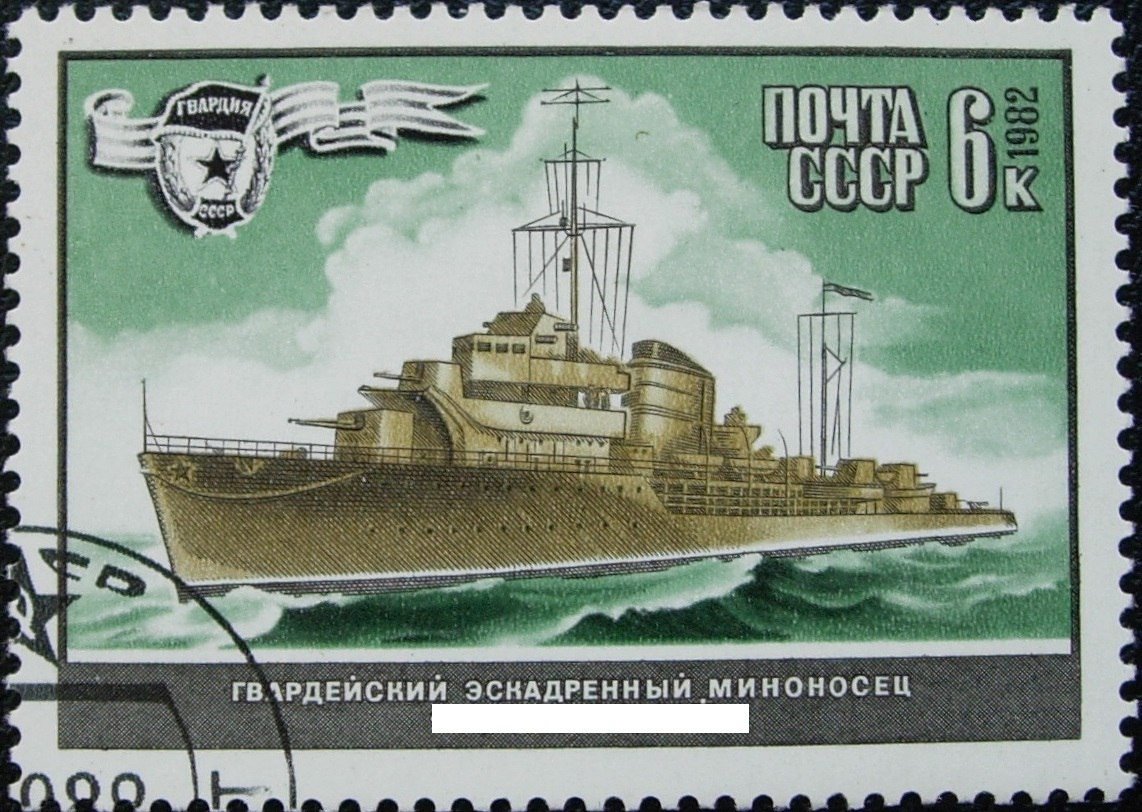
\includegraphics{chapter/ship/Secret_Grem_ship.jpg}}
  }
  На рисунке представлен самый известный советский \href{https://ru.wikipedia.org/wiki/Эскадренный_миноносец}{эскадренный миноносец} \href{https://ru.wikipedia.org/wiki/Эскадренные_миноносцы_проекта_7}{проекта 7}, удостоенный звания <<гвардейский>>, назовите его.
}


\section{Полнота свойств объектов военных кораблей}

Составим список кораблей (на русском языке), участвовавших в каких-либо конфликтах (см. листинг \ref{lst:ships_in_conflict_ru}).

\begin{lstlisting}[ language=SPARQL, caption={{\href{https://w.wiki/ghY}{Список кораблей, участвовавших в каких-либо конфликтах}}\protect\footnotemark}, label=lst:ships_in_conflict_ru, ]
#List of ships with countries and war conflicts in Russian
SELECT ?ship ?shipLabel ?countryLabel ?conflict ?conflictLabel
WHERE
{
  ?ship wdt:P31 wd:Q11446;        # instance of ship
        wdt:P137/wdt:P17 ?country;         # belongs to country
        wdt:P607 ?conflict.       # engaged in some conflict
  SERVICE wikibase:label { bd:serviceParam wikibase:language "ru". }
}
\end{lstlisting}
\footnotetext{Ссылка на SPARQL-запрос: \href{https://w.wiki/ghY}{https://w.wiki/ghY}, найдено \num{3586} кораблей в 2020 г.}

У военных кораблей, участвовавших в конфликтах, указывается свойство \href{https://www.wikidata.org/wiki/Property:P607}{conflict (P607)} (война/сражение). В то же время военные конфликты и военные операции, которые являются частью войн, являются разными понятиями. Объекты кораблей можно условно по делить на два типа:

\begin{enumerate}
  \item Объекты, у которых военные операции объединены с военными конфликтами. Например, у \href{https://www.wikidata.org/wiki/Q4148613}{эсминца Гремящий} девять войн/сражений. Такое большое число связано с тем, что корабль принял участие во многих \href{https://ru.wikipedia.org/wiki/Арктические_конвои}{арктических конвоях}, которые являются военными операциями.
  \item Объекты, у которых военные операции отделены от военных конфликтов. Например, у британского крейсера \href{https://ru.wikipedia.org/wiki/HMS_Trinidad_(1940)}{HMS Trinidad} участие в военной кампании и арктическом конвое указаны как часть Второй мировой войны с помощью квалификатора \href{https://www.wikidata.org/wiki/Property:P1012}{including (P1012)}. Таким образом, в Викиданных у этого крейсера указана одна война/сражение.
\end{enumerate}

Для первого типа объектов в скриптах с поиском у кораблей свойства \href{https://www.wikidata.org/wiki/Property:P607}{conflict (P607)} будет отображаться больше войн/сражений, чем при втором. Но в этом случае операция \href{https://ru.wikipedia.org/wiki/Одесская_оборона_(1941)}{Одесская оборона} будет стоять наряду с \href{https://ru.wikipedia.org/wiki/Великая_Отечественная_война}{Великой Отечественной войной}, хотя она является частью этой войны. В такой ситуации выводимые данные будут не точными.

% \label{question:ship_2}
% \marginnote{
%   Исходя из графика зависимости кораблей и военных действий (Рис. \ref{fig:ships_by_country_and_conflict}), на какую страну приходится больше всего значений войн, с которыми связаны корабли?
%   \begin{itemize}
%     \item СССР
%     \item Россия
%     \item Российская Империя
%   \end{itemize}
% }

% \label{question:ship_3}
% \marginnote{
%   Исходя из этого же графика, на какую войну приходится больше всего значений кораблей?
%   \begin{itemize}
%     \item \href{https://www.wikidata.org/wiki/Q159950}{Русско-японская война}
%     \item \href{https://www.wikidata.org/wiki/Q362}{Вторая мировая война}
%     \item \href{https://www.wikidata.org/wiki/Q254106}{Крымская война}
%   \end{itemize}
% }

Составим список кораблей (на русском языке) России, СССР или Российской Империи, участвовавших в каких-либо конфликтах (см. листинг \ref{lst:ships_in_war_ru}).

\begin{lstlisting}[ language=SPARQL, caption={{\href{https://w.wiki/koW}{Список кораблей России, СССР или Российской Империи, участвовавших в каких-либо конфликтах}}\protect\footnotemark}, label=lst:ships_in_war_ru, ]
#List of ship with countries and war conflicts in Russian
SELECT ?ship ?shipLabel ?countryLabel ?conflict ?conflictLabel
WHERE
{
  ?ship wdt:P31 wd:Q11446;        # instance of ship
        wdt:P137/wdt:P17 ?country;        # belongs to operator
        wdt:P607 ?conflict.       # engaged in some conflict
  
  { ?country wdt:P17 wd:Q34266 } UNION  # Russian Empire
  { ?country wdt:P17 wd:Q15180 } UNION  # Soviet Union
  { ?country wdt:P17 wd:Q159 }.         # Russia

  SERVICE wikibase:label { bd:serviceParam wikibase:language "ru". }
}
\end{lstlisting}
\footnotetext{Ссылка на SPARQL-запрос: \href{https://w.wiki/koW}{https://w.wiki/koW}. Найдено \num{86} кораблей в 2020 г.}
  

\begin{figure*}
  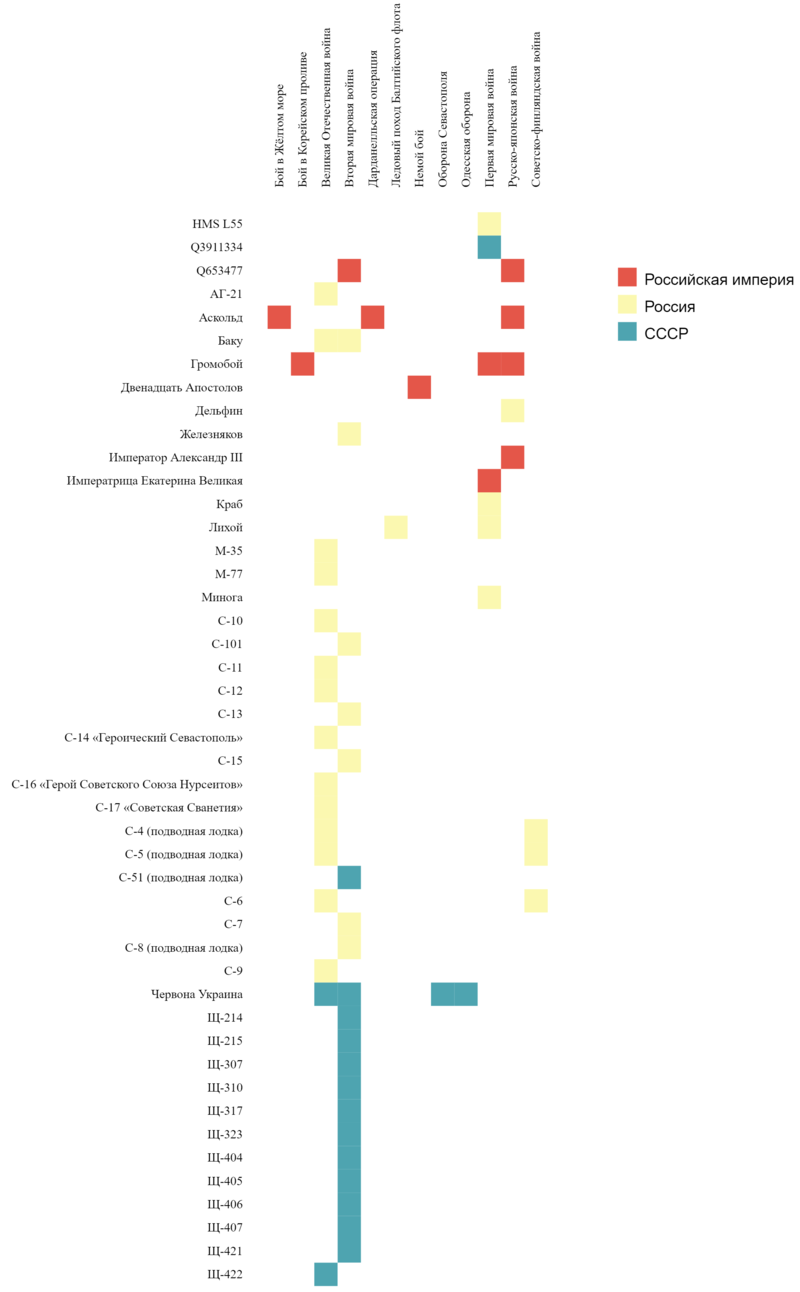
\includegraphics[width=\linewidth]{chapter/ship/Ships_by_country_and_conflict_ru.png}
  \caption{Фрагмент cписка кораблей, связанных с Россией и участвовавших в военных конфликтах, 2017 год. Из списка видно, что больше большая часть кораблей связаны с Россией и СССР, а также со Второй мировой или Великой Отечественной войнами.}%
  \label{fig:ships_by_country_and_conflict}%
\end{figure*}


\newpage
\section{Упражнения}

\begin{enumerate}
  \item Найти "корабль Гиннесса" (на выбор: самый большой, самый длинный, самый вместительный).
  \item Вывести фотографии тех кораблей, про которые снимали кино. Если таких не найдётся, тогда те корабли, о которых писали в книгах.
  \item Вывести\href{https://ru.wikipedia.org/wiki/Список_кораблей-музеев}{корабли-музеи}\footnotetext{\href{https://ru.wikipedia.org/wiki/Корабль-музей}{корабль-музей} -- судно или корабль, на котором размещена музейная экспозиция, посвящённая истории корабля, экипажа, событиям, в которых принимало участие судно, объект морского наследия.}
\end{enumerate}
